\documentclass[11pt,a4paper]{article}

\usepackage{hyperref}
\usepackage{graphicx}
\usepackage{amssymb}
\usepackage{amsmath}
\usepackage{amsthm}
\usepackage[margin=19mm]{geometry}
\usepackage{natbib}
\usepackage{bm}
\usepackage[toc,page]{appendix}
\usepackage{booktabs}
%\usepackage{url}
%\usepackage{fancyhdr}
%\usepackage{fancyvrb}
\usepackage{lscape}
%\usepackage{pdfsync}
\usepackage{rotating}
\usepackage{multirow}
\usepackage[nodisplayskipstretch]{setspace} \setstretch{1.5}
\let\oldv\verbatim
\def\verbatim{\par\setstretch{0.9}\oldv}
\usepackage[table]{xcolor}
\usepackage{algorithm,algorithmic}

%\renewcommand{\headrulewidth}{0.5pt} %Do not print a rule below the header
%\renewcommand{\footrulewidth}{0pt} %Do not print a rule above the footer

\bibpunct{(}{)}{;}{a}{,}{,}

%\renewenvironment{tabbing}{\linebreak \texttt \sl}{\linebreak}

\newcommand{\undertilde}[1]{\underset{\widetilde{}}{#1}}
\newcommand{\threeScript}[3]{
	\!\begin{smarray}{l}
  		{#1}\\ \hlx{s[-5pt]}
  		{#2}\\ \hlx{s[-5pt]}
  		{#3}
 	 \end{smarray}
}
\renewcommand{\baselinestretch}{1.5}
\setlength{\abovecaptionskip}{5pt}
\setlength{\belowcaptionskip}{-1pt}

\newtheorem{mydef}{Definition}

\floatname{algorithm}{Pseudocode}

\newcommand{\disfrac}{\displaystyle \frac}

\hypersetup{
    bookmarks=true,         % show bookmarks bar?
    unicode=false,          % non-Latin characters in Acrobat’s bookmarks
    pdftoolbar=true,        % show Acrobat’s toolbar?
    pdfmenubar=true,        % show Acrobat’s menu?
    pdffitwindow=false,     % window fit to page when opened
    pdfstartview={FitH},    % fits the width of the page to the window
    pdftitle={My title},    % title
    pdfauthor={Author},     % author
    pdfsubject={Subject},   % subject of the document
    pdfcreator={Creator},   % creator of the document
    pdfproducer={Producer}, % producer of the document
    pdfkeywords={keyword1} {key2} {key3}, % list of keywords
    pdfnewwindow=true,      % links in new window
    linktoc = page,
    colorlinks=true,       % false: boxed links; true: colored links
    linkcolor=blue,          % color of internal links
    citecolor=blue,        % color of links to bibliography
    filecolor=magenta,      % color of file links
    urlcolor=cyan           % color of external links
}

%###################################################################################################
%Writing starts here!!
%
%###################################################################################################

\begin{document}
\title{Introduction}
\author{Kevin Chang}
\date{\today}
\maketitle

%\tableofcontents
%\chapter{Quantitative Proteomics using MudPIT coupled with iTRAQ\textsuperscript{TM}}\label{chap:intro}

\section{Introduction}
All research studies require that the researchers conduct one or more experiments to make confident claims based on the study results. A thorough plan for an experiment is essential, and is important aspect of statistical theory called \emph{experimental design}. 

Many of the initial theories on experimental design were developed in the field of agriculture by \cite{Fisher1935}. However, most of these theories were developed with none or very little aid of computational power; thus, the view in the experimental design today is much differ from that of the 1930s. Therefore, the theory in the experimental design has also been developed rapidly with the advantage of the progression in the computers. 
 
There are several advantages of having a thorough experimental design. Firstly, it enhances the amount of information per experiment compared to an ad hoc approach. The second benefit is providing an organized approach toward analysis and interpretation of results; thus, facilitating communication between the statistician and the researcher \citep{Doyle2009}. 

The type of experiment that this thesis is focusing on is \emph{high-throughput biotechnologies experiment} (HTBE). The HTBE is the testing of multiple samples in a biological assay at the same time where each sample consists of large numbers of candidate molecules, such as genes or proteins \citep{Janzen2002}. Having a thorough experimental design becomes particularly important in HTBE, because these experiments can be very expensive to conduct. However, despite high-throughput biotechnologies have improved rapidly within a last decade; the statistical methods, for analysing the data generated from these technologies, are falling further behind \citep{Doyle2009}. Therefore, there is a need to improve in the theory for the design of HTBE. 

%There are many different families of designs exits in the published literature such as the reference design or loop design for the microarray experiments. 

For most of these HTBE, the responses of the experimental units to treatments cannot be measured directly in a single experiment, e.g.\ the gene expression level cannot be measured without the use of microarray technology. Thus, subsequent processing (Phase 2) of the initial (Phase 1) experiment is necessary in order for the measurements to be made. Another example is a proteomics experiment, which is the study of proteins. The Phase 1 experiment involves the organisms that are to be perturbed by the experimental conditions of interest. Since the abundance of proteins cannot be measured directly from the organisms, the Phase 2 experiment is required to measure the abundance of proteins in samples extracted from the organisms in the Phase 1 experiment. An example of the Phase 2 experiment is applying a multiplexing technique such as iTRAQ peptide labelling, coupled with liquid chromatography-mass spectrometry (LC-MS). Section~\ref{sec:proteomicExpt} describes in detail the biological background of the mass spectrometry based proteomics experiments. 

The purpose of this chapter is to establish some general understandings of the two-phase experiments. Section~\ref{sec:introTwoPhase} to \ref{sec:brien2011} describe how the methods surrounding the two-phase experiments have evolved over the last few decades. The biological background of the proteomics experiments is explained in Section~\ref{sec:proteomicExpt}. Section~\ref{sec:overview} briefly describes the overview of this thesis.

%This will aid in the understanding of the two-phase experiment which can also be employed as a part of important idea in the designing two-phase experiment.

\section{The introduction of two-phase experiments by McIntyre}
\label{sec:introTwoPhase}
Two-phase experiments were first introduced by \cite{McIntyre1955}. He used an real example that investigated the effects of four light treatments on the synthesis of tobacco mosaic viruses in the tobacco leaves. In the Phase 1 experiment, two $4 \times 4$ square arrays are made up by eight plants and four leaves within plants. Four different treatments are then assigned to the plants and leaves in such way where each treatment occurs only once within each row and column in each of two $4 \times 4$ square arrays. This assignment is also known \emph{Latin square design} \citep{Bailey2008}. Hence, there are 32 observations from the Phase 1 experiment. However, the virus contents from each leaf cannot be measure directly in the Phase 1 experiment. Hence, the virus content of the leaves from the plants of the Phase 1 experiments, referred to as \emph{test plants}, was assayed by expressing sap using a completely different set of plants, referred to as \emph{assay plants}, for the Phase 2 experiment. 

In the Phase 2 experiment, 16 assay plants and four leaves within each assay plants were used. In addition, each leaf is further subdivided into two half leaves, which allows to measure 128 samples. Given that there are 32 samples from the Phase 1 experiment, each sample are replicated four times for the measurement in the Phase 2 experiment. For the assignment of the Phase 2 experiment, four $4 \times 4$ square arrays are made up by the 16 plants and four leaves with plants. Furthermore, since each leaf is further subdivided into two half leaves, the Phase 2 design can be expressed as two sets of Latin squares designs superimposed to each other, which also known as  \emph{Greaco-Latin square design}. This experiment is a good example of the two-phase experiment where there are two different experimental designs required; the first design is to prepare a set of samples and second design is to measure bio-substances of interest from each of these samples. 

The analysis of variance (ANOVA) table were used which explain the sources of variation that were introduced from the two-phase experiment. For each source of variation, the \emph{sum of squares} (SS) can be computed from the experimental data and the \emph{expected mean squares} (EMS) can be derived solely from the experimental design. EMS is the linear combination of \emph{variance component}, commonly denoted by $\sigma_{i}^2$ from factor $i$, which indicates the contribution of the variation from different factor. Hence, ANOVA table is essential tool for dissecting the different variation in any experiment and can useful for the complicate experiment involves with many factor, such as two-phase experiments. 

\cite{McIntyre1955} presented two important principles for designing the two-phase experiment. The replication of the treatment in the Phase 1 experiment is essential, because  the statistical test of the treatment effects for the Phase 1 experiment should be achievable separately from the Phase 2 experiment. The replication in the Phase 2 experiment is not necessary unless there is uncontrollable variation introduced from the Phase 2 experiment. The main objective in the theory of two-phase experiment is the relationship between the factors from the Phase 2 experiment and the Phase 1 experiment. For the example experiment mentioned, the treatment are replicated four times in the Phase 1 experiment. In addition, each sample from the Phase 1 experiment is further replicated four times before assigning to the Phase 2 experiment. 

\cite{McIntyre1955} concluded with three important concepts. Firstly, he demonstrated that the different two-phase design combinations can induce different error variances for the treatment effects, because different designs will result in the different combinations of the variance components. Secondly, based on the example experiment, with doubling in the replication in the Phase 2 experiment, the error variance for the treatment effects is reduced by only $19\%$; however, the amount time for complete the experiment is doubled. Finally, if there is no treatment replication within the Phase 1 experiment, then the error variance for the treatment effects will be inflated. This is because the error variance will include the variation of between leaves within plants from both Phase 1 and Phase 2 experiments. 

In summary, the construction of the ANOVA table with EMS is shown to be essential for illustrating the linear combination of the variance components. This is because it allows the estimation of the error variance for the treatment effects. However, the method in constructing the ANOVA table with EMS was not mentioned by \cite{McIntyre1955}.
 
\section{Non-orthogonal structure of the two-phase experiment}
\cite{Curnow1959} revisits the theory of two-phase experiments, where he produced a new ANOVA table of the overall analysis for \citeauthor{McIntyre1955}'s last example. The new ANOVA table is better than the ANOVA presents by \cite{McIntyre1955}, because it shows every SS and the corresponding \emph{degrees of freedom} (DF) for the light treatment experiment. In addition, the ANOVA table also shows the separation of the treatment effects into two sources of variation. The first  treatment effects estimate contains the variance components of between leaves from the assay plants whereas the second treatment effects estimate does not. \cite{Curnow1959} terms these first and second estimations of the treatment effects are \emph{sums} and \emph{differences} analyses, respectively, which are equivalent of \emph{inter} and \emph{intra}-block analyses, respectively. \cite{Curnow1959} then showed how to combine the inter- and intra-block analyses using the weights computed from the variance of treatment estimate. Nevertheless, the new ANOVA table, given by \cite{Curnow1959}, emphasised in the combining the estimates from the intra- and inter-block analyses which provides a first improvement in developing a better analytic procedure for the two-phase experiments. 

\cite{Wood1988} then discussed the non-orthogonal block structure of the two-phase experiments which is an extension from the theory described by \cite{Curnow1959}. The non-orthogonal structure is typically occurred when the treatment effects that can be estimated from both inter- and intra-block analyses, as seen from example from \cite{McIntyre1955} and \cite{Curnow1959}, i.e.\ non-orthogonal treatment structure. Similarly, the non-orthogonal block structure can also occur when the block factor from the Phase 1 experiment is confounded with the block factor of the Phase 2 experiment for the two-phase experiment. The amount of orthogonality can be measured by the \emph{efficiency factor} which is the amount of treatment information presents for the intra-block analysis \citep{Yates1936}. Thus, the efficiency factor should also be used to measure the amount of block information for the cases of non-orthogonal block structure. 

The non-orthogonal structure can occur in two different ways. The first way is when the DF of block effects from the Phase 1 experiment are split to inter- and intra-blocks. This can be shown in the ANOVA table given by \cite{Curnow1959} where the total of 6 DF associated with the leaf positions of the test plants is split into 2 SS where both SS are estimated with 3 DF. This first SS is confounded with the whole leaves of the assay plants and the second SS is orthogonal to the whole leaves of the assay plants. The efficiency factor for both SS can be shown to be 100\%. The second way is where the DF of block effects from the Phase 1 experiment stay intact. This can be shown in the artificial example by \cite{Wood1988} where all 3 DF associated the units SS of the Phase 1 experiment are estimated in both Between and Within Blocks. The amount of the separation for this case is then measured by the efficiency factor. Both types of confounding should be minimised, because it can affect whether the test for the treatment effects can be conducted.   Chapter 3 and 4 describes in finding the optimal two-phase design which will further discuss the non-orthogonal treatment and block structures. 


%McIntyre used Latin square analysis to estimate the treatment effect which is equivalent of taking the un-weighted estimate the treatment effects. However, based on the new ANOVA table presented, the sums and differences analyses are equivalent of inter-block and intra-block analyses, respectively, that are arise in the analysis of an incomplete block design. If the variances in the treatment estimates from the inter-block and intra-block analyses are very different, then Curnow believed that weighting the estimates according to treatment variances would be a better method. Thus, the treatment estimate is given by 
%\begin{equation}\label{eq:weightTrtEst}
%\hat{\tau} = w \hat{\tau}_{inter} + (1 - w)\hat{\tau}_{intra} ,
%\end{equation}
%where $w$ denotes the weight, and $\overline{\tau}_{inter}$ and $\overline{\tau}_{intra}$ denotes the treatment estimates from the inter-block and intra-block analyses, respectively. Since the variance of treatment estimate can be expressed as 
%\[
%\mathrm{Var}[w  \hat{\tau}_{inter} + (1 - w)\hat{\tau}_{intra}] = w^2 \mathrm{Var}(\hat{\tau}_{inter}) + 2 w (1-w)  \mathrm{Cov}(\hat{\tau}_{inter}, \hat{\tau}_{intra}) + (1-w)^2 \mathrm{Var}(\hat{\tau}_{intra}), 
%\]
%which is minimised by choosing 
%\begin{equation}
%w = \frac{\mathrm{Var}(\hat{\tau}_{intra}) - \mathrm{Cov}(\hat{\tau}_{intra}, \hat{\tau}_{inter})}{\mathrm{Var}(\hat{\tau}_{intra}) + \mathrm{Var}(\hat{\tau}_{inter}) - 2\mathrm{Cov}(\hat{\tau}_{intra}, \hat{\tau}_{inter})}.
%\end{equation}

%For the variance components present in the intra-block and inter-block analyses, \cite{Curnow1959} also used the weighted estimates by combining the variance component estimates from these two analyses. The weight is also computed by minimising the variances of the variance component estimate.

%However, for the example given by McIntyre, the \citeauthor{Curnow1959}'s method did not produce a very different estimation for both treatment effects and the variance components comparing to \cite{McIntyre1955}. Nevertheless, the new ANOVA table, given by  \cite{Curnow1959},emphasised in the combining the estimates from the intra-block and inter-block analyses which provides a first improvement in developing a better analytic procedure for the two-phase experiments. 

\section{Constructing the analysis of variance table}
Neither publications by \cite{McIntyre1955} and \cite{Curnow1959} did not mention on how their ANOVA tables were determined, particularly for the complex experiments such as two-phase experiments. Hence, \cite{Brien1983} presents a generalised procedure in determining the ANOVA table. Note that the ANOVA presented only consists of sources of variation and the corresponding DF. This section briefly describes the procedure by \cite{Brien1983}, which contains some basic terminologies for designing experiments.

Before constructing the ANOVA table, the overall structure of the experiment has to be determined. The first step is to identify the factors in the experiment and the observational unit. The observational unit is the smallest unit of the experiment \cite{Bailey2008}. The second step is to divide the factors into different sets; these sets are also known as \emph{tiers}. The first tier consists of the factors which would jointly identify the observational unit if no randomisation had been performed. These factors are also known as block factors by \cite{Nelder1965A}. The factor at the second tier are those level combinations have been directly associated with the level combinations of the factor at the first tier, this associated is usually known as \emph{randomisation}. Thus, the factor at the second tier are also known as treatment factors by \cite{Nelder1965B}.
 
The last step is to determine the relationship between the factors within each tier. \cite{Wilkinson1973} developed a symbolic syntax for representing the relationship between the block factors, i.e.\ \emph{block structure}, and treatment factors, i.e.\ \emph{treatment structure}, in an experiment. \cite{Brien1999} referred to this representation as a \emph{structure formula}. \citeauthor{Wilkinson1973}'s syntax was originally developed to generate and analyse the ANOVA models in the GenStat statistical analysis program, although it is now widely used in many statistical packages. Two basic operations, that are described by \cite{Wilkinson1973}, for representing block and treatment structures, namely \emph{crossing} denoted by an asterisk, $*$, and \emph{nesting}, denoted by a slash, $/$. 

For the two-phase experiment, there will be three tiers of factors, two set of block factors and one set of treatment factors. Hence, two-phase experiments also known as \emph{multi-tiered experiment}. The tier 1 and 2 consist of block factors from the Phase 2 and 1 experiments, respectively. The tier 3 contains the treatment factors of the overall experiments.  

Once the structure formula for every tier of experiment is determined, the ANOVA table can be derived. First step is to expand the structure formulae for each tier which gives a set of terms based on the rules described by \cite{Wilkinson1973}. The terms from the first tier forms a initial structure of the ANOVA table. The terms from the second tier are included in the table under the terms of the first tier with indentation, only if the two terms from different tiers are confounded with each other. The confounding between the terms can be examined from the contrasts generated from each term. For the two-phase experiment, there is an additional tier. Therefore, the terms from the tier 3 are included under the terms of tier 1 or 2 with another indentation, if there is confounding between the terms from the two different tiers. For a more detail description of these procedures see \cite{Brien1983}.

\cite{Brien1983} concluded with idea of the randomisation procedures between the factors of different tiers can alter the relationship of factors within each tier. Consider an experiment arranged by the row-column design; thus, the relationship between the row and column factors should \emph{crossed}. However, if the treatment factor can only be randomised to the column factor; then, the treatment factor becomes confounded with the column factor. Consequently, the relationship between the row and column factors is then \emph{nested}. In summary, the experimental structure depends on the innate physical structure as well as how the randomisation procedure is employed. 


\section{Complicated two-phase experiments}
The rules described in \cite{Brien1983} can be difficult to apply for a complicated two-phase experiments with non-orthogonal structure. This is because the confounding between the terms of different tiers can be hard to examine with just their contrasts. Thus, \cite{Brien1999} described an algorithm which consists of fitting terms into the model by two types sweeping operations.  The given algorithm can be used to construct the ANOVA table for any single- or two-phase experiment. 

The sweeping operations were originally discussed by \cite{Wilkinson1970} and \cite{Payne1977}. The first sweep operator is the \emph{pivotal sweep} which involves the effects that are placed into a unit length vector. This means the data vector is projected from one vector subspace to another vector subspace, where each vector subspace is corresponding to the each term expanded from the structure formula. Thus, this sweeping operator can be expressed as 
\begin{equation}
E_i Q_i
\end{equation}
where $E_i$ and $Q_i$ are the efficiency factor and orthogonal projector matrix associated with term $i$ from the expanded structure formula. The second sweep operator is called \emph{reanalysis sweep}. This sweep is performed when terms from two different structure formulae that are non-orthogonal to each other, i.e. non-orthogonal block or treatment structures. Hence, before performing the pivotal sweep to the next term; the effect from the current term is removed using the reanalysis sweep. This sweeping operator can be express as 
\begin{equation}
I - E_i Q_i
\end{equation}
where $I$ is the identity matrix. Since the methods are based on the projection of vectors, the reanalysis sweep is based on the \emph{Pythagorean theorem}, which is the subtraction of two vectors to obtain the resultant vector with orthogonal complement.

\cite{Brien1999} addressed this algorithm can be extended for the two-phase experiment by performing a extra series of sweeps for terms from the third structure formula. These two sweeping operators play a vital part in the decomposition of the raw data and the computation of the sum of square for the ANOVA table. This is further discussed in Chapter 2 of the thesis.

\section{Moving toward the high-throughput biotechnology}
\cite{Jarrett2008} demonstrated how the two-phase experiment can be applied on the gene expression two-colour microarray experiments. The Phase 1 experiment requires some experimental design to prepare the two more condition for comparison. This experiment then provides some physical materials, i.e.\ mRNA, for the Phase 2 experiment. Another experimental design is required for the Phase 2 experiment on how the samples from the Phase 1 experiment is allocated to different dyes and arrays. In the end, the Phase 2 experiment generate some numerical values that need to be analysed. 

\cite{Jarrett2008} demonstrated on how to assess the effectiveness of the estimates using the effective degrees of freedom (EDF). The EDF is computed by the first two moments of an approximating chi-square distribution. This thesis will use the EDF to compare the competing designs which is presented in the Chapter 5.


\section{Works by Brien and Bailey} 
\cite{Brien2006b} describes how the randomisation can be achieved for the two-phase experiments. Randomisation is a important concept in the experimental design which involves how the one set of objects can be randomly assignment to another set of objects. As \cite{Brien1983} pointed out the randomisation can affect the structure of the experiments. The main purpose of randomisation is to enable to researcher to obtain the data set with minimal systematic biases. 

Since two-phase experiment involves three tiers of factors; the randomisation procedure is perform multiple times when assigned the factors between different tiers. Thus, \cite{Brien2006b} called \emph{multiple randomisation}. 

\cite{Brien2006b} then compared and contrasted six types of multiple randomisations. These are composed, coincident, independent, double, randomised-inclusive and un-randomised-inclusive multiple randomisations. These six different multiple randomisations are differ in the direction of the randomisation as well as how the terms in different tier are interact with each other. For a more detail description of these multiple randomisations see \cite{Brien2006b}.  

\cite{Brien2009, Brien2010} then published two papers on the aspects of orthogonal decomposition of the data space for the two-phase experiment for different type of multiple randomisations.

Two different notations in representing the  orthogonal decomposition of the data space are introduced by \cite{Brien2009}. Given that two sets of orthogonal matrices are denoted by $\mathcal{P}$ and $\mathcal{Q}$, the matrix set $\mathcal{P}$ decomposed by the matrix set $\mathcal{Q}$ is expressed by
\begin{equation}
\mathcal{P} \rhd \mathcal{Q}.
\end{equation}
Given that $P \in \mathcal{P}$ and $Q \in \mathcal{Q}$, 
\begin{equation}
P \rhd Q =  E_{PQ}^{-1}PQP
\end{equation}
where $E_{PQ}$ denotes the efficiency factor of $P$ decomposed by $Q$. Another expression 
\begin{equation}
P \vdash \mathcal{Q}
\end{equation}
stands for $P$ orthogonal to $ \mathcal{Q}$ or the residual of $\mathcal{Q}$ in $P$. Thus, 
\begin{equation}
P \vdash  \mathcal{Q} = P - \sum_{Q \in \mathcal{Q}} P \rhd Q
\end{equation} 
where $\sum_{Q \in \mathcal{Q}}$ denotes summation over $Q$ in $\mathcal{Q}$. The illustration of the decomposition for the two-phase experiment is comprised of these two notations of decompositions, $\rhd $ and $\vdash$. 

Since different multiple randomisations have different order of randomisation, \cite{Brien2009, Brien2010} showed that it can also affect the ordering of the orthogonal  decomposition between the terms of different tiers. In addition, knowing the randomisation procedure initially, it allows the researchers to recognise hows the terms are confounded with each other between the tiers, which can simplify the researchers to deduce the decomposition procedure for the given experiment. However, categorising the experiment on the type of multiple randomisations given in \cite{Brien2006b} is not always straightforward, because the confounding between the terms of different tiers may not always be obvious; especially for the complicated two-phase experiments. 

Therefore, I believe the left to right orthogonal decomposition procedure can be applied for any two-phase experiment, without any prior knowledge of how the randomisation procedure is achieved. This is because the confounding between the terms of different tiers can always be resolved through the decomposition procedure. The left to right orthogonal decomposition procedure consists of two steps. The first step is to decompose the terms from the block tier of Phase 1 experiment to the terms from the block tier of the Phase 2 experiment. The second step is to decompose the terms from the treatment tier to the resultant products of the first decomposition step. Chapter 2 utilised this decomposition procedure for any single or two-phase experiment without any prior knowledge of how the randomisation procedure is achieved. 

Furthermore, \cite{Brien2009, Brien2010} only considered the balanced designs, which have a set of identical efficiency factors for every DF of the corresponding block or treatment effects. Chapter 3 and 4 of the thesis presents some optimal designs that are not balanced; which can be confusing to represent in the ANOVA table.  
 
\section{Recent work by Brien}
\label{sec:brien2011}
A more recent paper by \cite{Brien2011} discussed a systematic approach in designing the two-phase experiment. This paper only considers the design with the orthogonal structure. Some principles described are used as the basis in developing the method of finding the optimal design in Chapter 3 and 4 of the thesis. 

The first principle is to formulate the skeleton ANOVA table using this factor-allocation diagram. The factor-allocation diagram is the randomisation diagram as discussed in \cite{Brien2006b}. \cite{Brien2011} presents a list of rules for calculating the EMS of the ANOVA table. However, these rules can still be laborious to follow for the experiment with many treatment and block factors. Chapter 2 of this thesis presents an R package which automatically generate the ANOVA table with the EMS for any single or two-phase experiment. 

\cite{Brien2011} then discussed some fundamental principles for designing the two-phase experiment. Firstly, the block factor of the Phase 1 experiment with the highest variation, but orthogonal to treatments, should be confounded with the block factor of the Phase 2 experiment containing the highest variation. This situation can be observed in Chapter 4 of the thesis in finding the optimal design where the Phase 1 experiment is randomised block design. 

Furthermore, the treatment factors from either Phase 1 or Phase 2 experiment should be assigned with the random factor of Phase 2 experiment with the smallest variation. Thus, the test for the treatment effects is conducted with the minimal experimental error. The treatment effect can be confounded with multiple random effects of Phase 2 experiment which is caused by the non-orthogonal treatment structure; but, this was not discussed by \cite{Brien2011}. Chapter 3 and 4 of the thesis describe some designs with the non-orthogonal structure. 

\section{Proteomic experiment}
\label{sec:proteomicExpt}
Throughout this thesis, the proteomic study is used as a principle example for the hight-throughput experiment. Proteomic studies require the use of a combination of technologies, coupled with database searching, for the identification and quantification of the proteins within a target cell, tissue or biofluid. The purpose of this section is to provide a detailed description of these identifications and measurements are made. By understanding the data generation process, we hope to also have a better understanding of how to design proteomics experiments using the technologies described. Thus, Section~\ref{subsec:protein} provides a detailed introduction to proteins and some of their properties, and defines what is meant by a proteome. Section~\ref{subsec:MudPIT} describes the process of separating a complex protein mixture into smaller subunits so that high resolution measurements can be made of the proteins’ constituent components by the mass spectrometer. Section~\ref{subsec:iTRAQ} describes a recent protein labelling technology which enables the simultaneous analysis of multiple protein complex protein mixtures. 

\subsection{Proteins and the Proteome}
\label{subsec:protein}
Proteins are one of the major macromolecules within a biological system which contribute to every process of a living system and are considered as the essential building blocks of life. They are constructed from a chain of amino acids, joined together by peptide bonds~\citep{Eidhammer2008}. The amino acid sequences are derived from the genes in the cell nucleus via the processes of transcription, where DNA is copied to mRNA, and then translation, where messenger RNA (mRNA) is decoded into proteins (see Figure~\ref{fig:processes}). Furthermore, a pre-mRNA may undergo alternative splicing as part of the post-transcription process and can, therefore, produce more than one protein sequence. This makes the study of protein expression functionally more relevant than the study of mRNA, transcription also known as \emph{gene expression}.

A protein can be digested into smaller units, or peptides, which comprise subsequences of the amino acids in the intact protein. Hence, proteins are also termed polypeptides. The peptides are produced by enzymatic digestion of a whole protein. An example of one such enzyme is \emph{trypsin}~\citep{Eidhammer2008}. 

\begin{figure}[hbt]
\centering{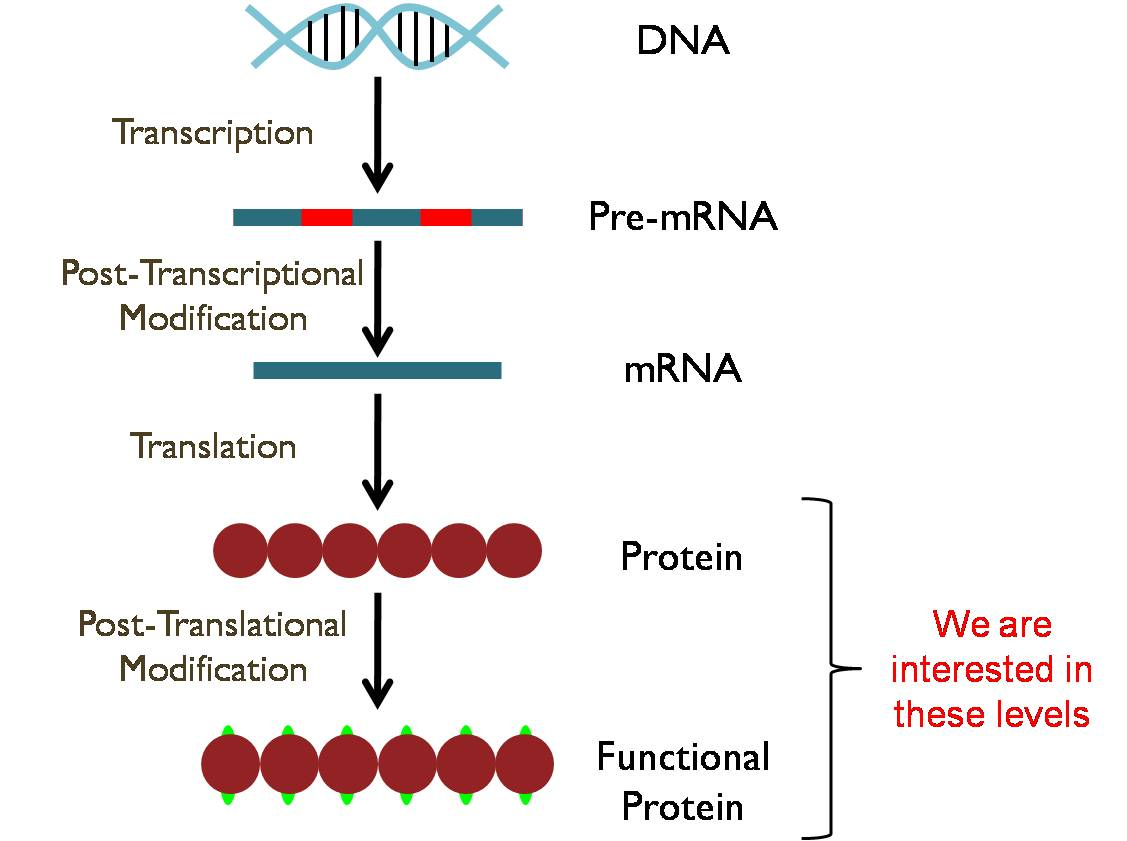
\includegraphics[scale=0.55]{image/processes.jpg}}
\caption{Basic biological processes of producing functional proteins from DNA.}
\label{fig:processes}
\end{figure}

The proteome is the entire complement of proteins expressed by the genome in a cell or tissue or bio-fluid of an organism at a given time point under a well-defined set of conditions \citep{Boehm2007}. A protein's function corresponds to when and where it is expressed. Hence, identification and localisation of many more unknown proteins and their functions is the ultimate goal of proteomic research. 

There are many ways to study proteins. For example, a protein's physical structure can be studied by X-ray crystallography~\citep{Blow2002}, protein-protein interactions are studied by the yeast two-hybrid system~\citep{Fields1989}, and the abundance of an individual protein under a defined condition can be studied using isotopic-labelling. The latter is also referred to as \emph{quantitative proteomics}. An example of the technologies for measuring the protein abundances is using Multi-dimensional Protein Identification Technology (MudPIT) in conjunction with isobaric Tags for Relative and Absolute Quantitation (iTRAQ\textsuperscript{TM}). 

\subsection{Multi-dimensional Protein Identification Technology} \label{subsec:MudPIT}
MudPIT refers to the process of separating a protein complex or peptide mixture, using the different properties of amino acids, into usually three orthogonal dimensions~\citep{Washburn2001}. Typically, the first separation is by charge, using \emph{strong cation exchange chromatography} (SCX), followed by hydrophobicity, using \emph{reversed phase liquid chromatography} (RPLC). The third dimension of separation is by mass and is carried out by \emph{mass spectrometry} (MS). This reduces the sample complexity and enables high throughput protein analysis. Hence, each  MudPIT \emph{run} is comprised of these three steps of separation.

There are some limitations associated with MudPIT. The variation in signal intensity between different MudPIT runs can be large, making the comparisons of peptide or protein abundances between samples difficult. This limitation has been resolved with the introduction of iTRAQ\textsuperscript{TM} labelling which enables the simultaneous analysis of up to eight distinct protein digests within a single MudPIT run.

\subsection{iTRAQ\textsuperscript{TM} for Protein Quantitation}\label{subsec:iTRAQ}
In its initial format, introduced by \cite{Ross2004}, iTRAQ comprised of four isobaric tags, each consisting of a reporter group, a balance group and a peptide reactive group. The reactive group binds the N-terminus at the start of each peptide, and, if the peptide contains lysine residues (i.e. amino acid) then, also on the lysine's side chain. The m/z values of the four reporter groups range in value from 114 to 117, with corresponding balance group values ranging from 31 to 28, respectively. Thus, each of four tags has an identical total m/z value of 145, making them isobaric. This enables identical peptide species, differentially labelled with the four tags, to be indistinguishable with respect to the intact mass of the peptide when selected for MS/MS~\citep{Ross2004}. For MS/MS, the relative abundances are determined from the reporter ion signals at m/z value of 114, 115, 116 and 117 on the \emph{mass spectrum}. A mass spectrum is a graphical representation of the peptides and peptide fragments based on their m/z value and abundances, and is generated for both phases of MS/MS. Thus, the four different labels allow four different samples to be simultaneously analysed~\citep{Ross2004}.
  
\begin{figure}[htb]
\centering{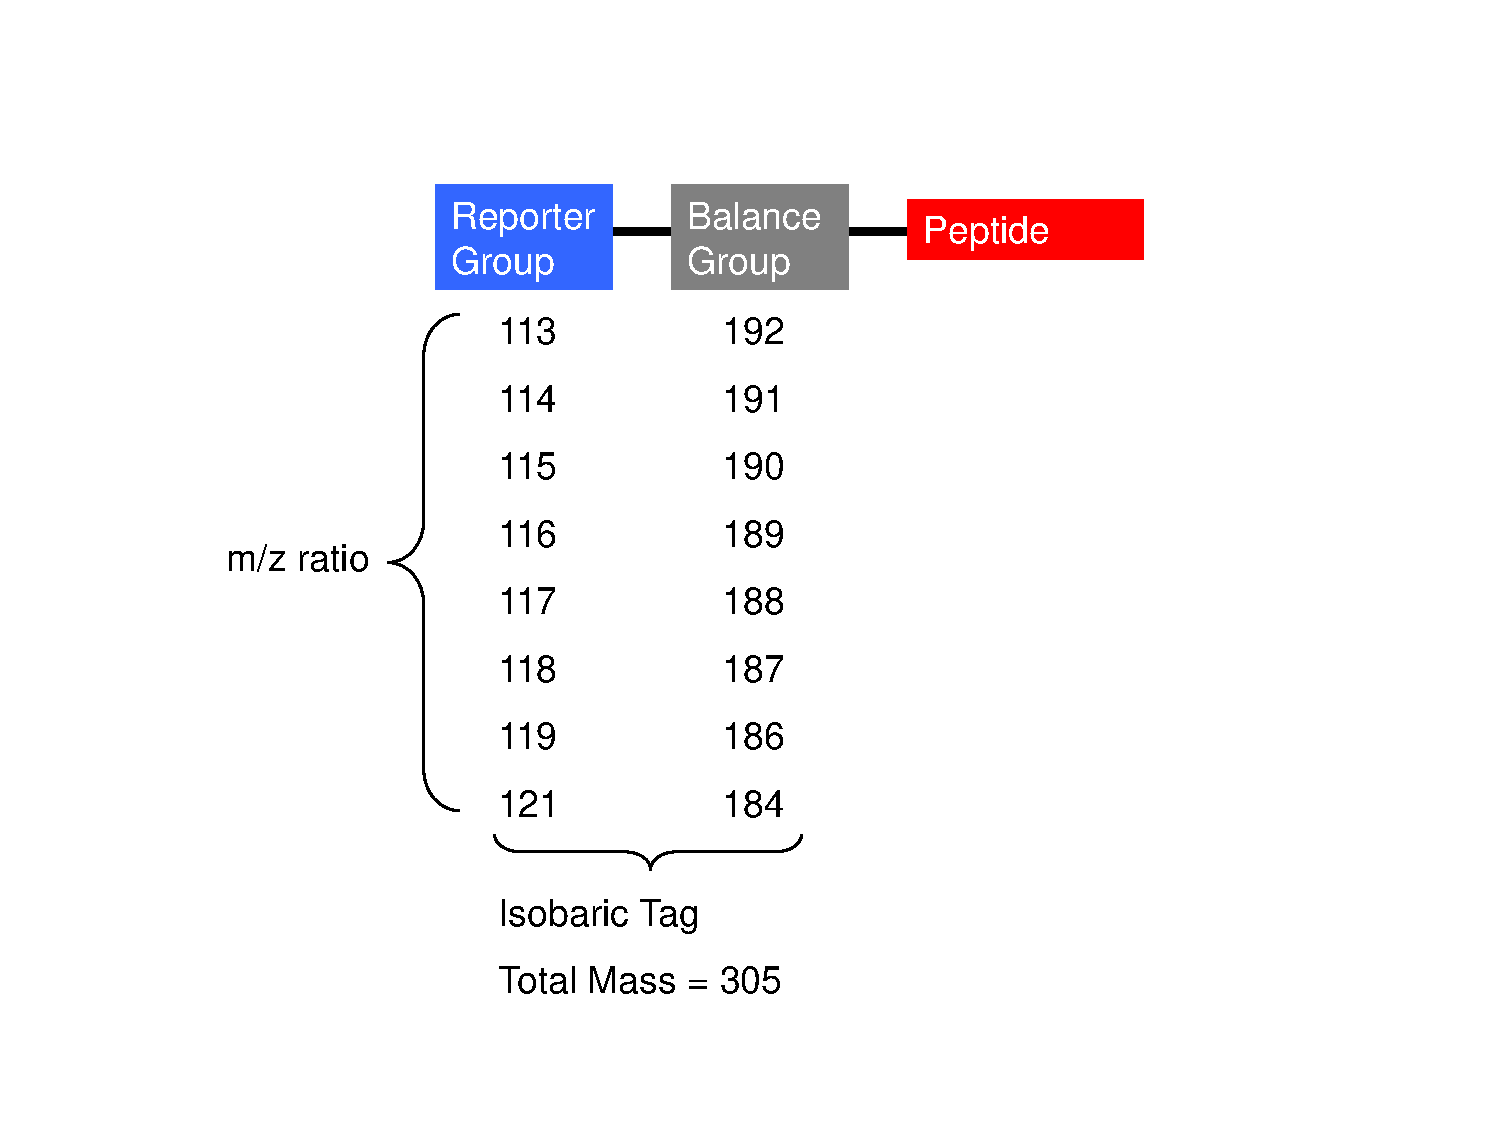
\includegraphics[scale=0.6]{image/iTRAQtags.pdf}}
\caption{Structure of 8-plex-iTRAQ\textsuperscript{TM} tags showing reporter and balance group masses measured in m/z~\citep{Choe2007}.}
\label{fig:8-plex}
\end{figure}

\cite{Choe2007} described a new multiplexing strategy, using the same concept as the four-plex iTRAQ\textsuperscript{TM} system, which allows the simultaneous analysis of up to eight distinct protein samples (see Figure~\ref{fig:8-plex}). This scheme has the reporter ion signals located at m/z values of 113, 114, 115, 116, 117, 118, 119 and 121. A label for an m/z of 120 is not used because this has the same mass as the phenylalanine immonium ion~\citep{Pierce2008}.   

\section{Overview}
\label{sec:overview}
The main goal of this thesis is to develop some general theories in two-phase experiments. These thesis can be divided into three main parts as follows. 

The first part, described in Chapter 2,  generalised the decomposition method for two-phase experiments with the construction the ANOVA table. As mentioned by \cite{Brien2011}, the ANOVA tables with the EMS for two-phase experiments are valuable in comparing the properties of different two-phase experimental designs. However, there is no any tool can automatically generate a such table. An R package called infoDecompuTE is presented which allows the researchers to generate the ANOVA table with EMS by entering any single or two-phase experimental design. Thus, this package will not only allow researchers to determine whether or not a valid F-test can be conducted from any given design; it will also enable the researchers to study the decomposition of the raw data into different strata and sources of variation.

For a given set of design parameters, there are often many ways to allocate the samples collected from the Phase 1 experiment to the block factors in the Phase 2 experiment. Chapter 3 and 4 show that the objective function defined can identifies the best allocation in terms of allowing a formal test of treatment effects to be conducted with the highest efficiency factor. The objective function is optimised using a simulated annealing algorithm. Furthermore, the objective function presented can be used to find the optimal two-phase design, where the Phase 1 experiment is arranged in a completely randomised design and randomised block design, respectively. The Phase 2 experiment is in a randomised block design. This type of two-phase experiment structure is typically for the high-throughput biotechnology experiment. In addition, an improved version of the SA, which is more efficient, is presented.

Finally, Chapter 5 describes a method in estimating the variance components and the effective degrees freedom (EDF) for the two-phase experiments. The restricted maximum likelihood method is described in estimating the variance components form the two-phase experiment with non-orthogonal block structures. EDF, computed from different variance component estimates, will then be used to compare the different optimal two-phase design found in Chapter 3 and 4. These specific examples will be used to elucidate the properties of different candidate designs and to work more towards a general theory of two-phase experiments.  


\bibliographystyle{apalike}
\bibliography{Reference/ref}

\end{document}
